\documentclass[../main]{subfiles}
\begin{document}

\graphicspath{{../figures/chap1/}}

\section{先行研究}
\label{sec:intro_previous-research}
地盤強度を取得する先行研究として,\refsubsec{subsec:intro_presearch_direct}で直接測定する手法,\refsubsec{subsec:intro_presearch_indirect}で間接的に推定する手法について述べる.
\subsection{地盤強度の直接測定}
\label{subsec:intro_presearch_direct}
建設機械の走破性を判定するために用いられる,地盤強度を示す指標の1つとしてコーン指数が挙げられる\citeen{Mulqueen1977} \citeen{Perumpral1987}.
コーン指数とは,コーンペネトロメータと呼ばれる棒状の測定器具を地面に挿入し,その際に発生する土の抵抗をダイヤルゲージで測定することで得られる値である.
コーンペネトロメータを\reffig{fig:cone_penetrometer}に示す.
土の抵抗力が大きいほど地盤の支持力が大きく,建設機械の走破性が高いと言えるので,コーン指数が大きいほど建設機械の走破性が高いと判定できる.
\reftab{tab:traffic_cone_index}が示すように,各建設機械の走行に必要とされているコーン指数は既にわかっている.
測定,または推定した地盤のコーン指数と\reftab{tab:traffic_cone_index}とを照らし合わせて建設機械の走破性を判定することが可能である.

コーン指数の測定は通常人の手でコーンペネトロメータを地面に挿入することで行う.
しかし,広範囲の地盤に対して人の手で測定を行うことは多くの時間と手間がかかる.
また,災害現場では二次災害が発生する可能性もあり,人が立ち入ることは危険が伴うので,人が現場に行き,測定などの作業を行うことなく,災害現場での建設機械の走破性判定を行える必要がある.

無人で走破性を判定する先行研究では,コーン指数を測定するための器具をロボットに搭載し,そのロボットを遠隔操作してコーン指数を測定する手法が提案されている\citeja{Huruya2016} \citeen{Chhaniyara2012} \citeen{Zacny2010}.
これらの手法では,人による測定をロボットで代替することで,人が現場に行くことなくコーン指数の測定を行うことを可能としている.
しかし,これらの手法で用いられる測定器具はコーンペネトロメータと同様に棒状であり,コーン指数測定は貫入点ごとに行われる.
そのため,災害現場全体についてコーン指数を測定するには時間がかかり,迅速さが求められる災害の復旧作業には適さない.
また,ロボットが測定場所まで移動する必要があるため,途中に段差などのロボットが踏破できない場所があり,ロボットの移動が不可能である場合にはコーン指数の測定自体が行えなくなるという問題点もある.

\begin{figure}[t]
    \centering
    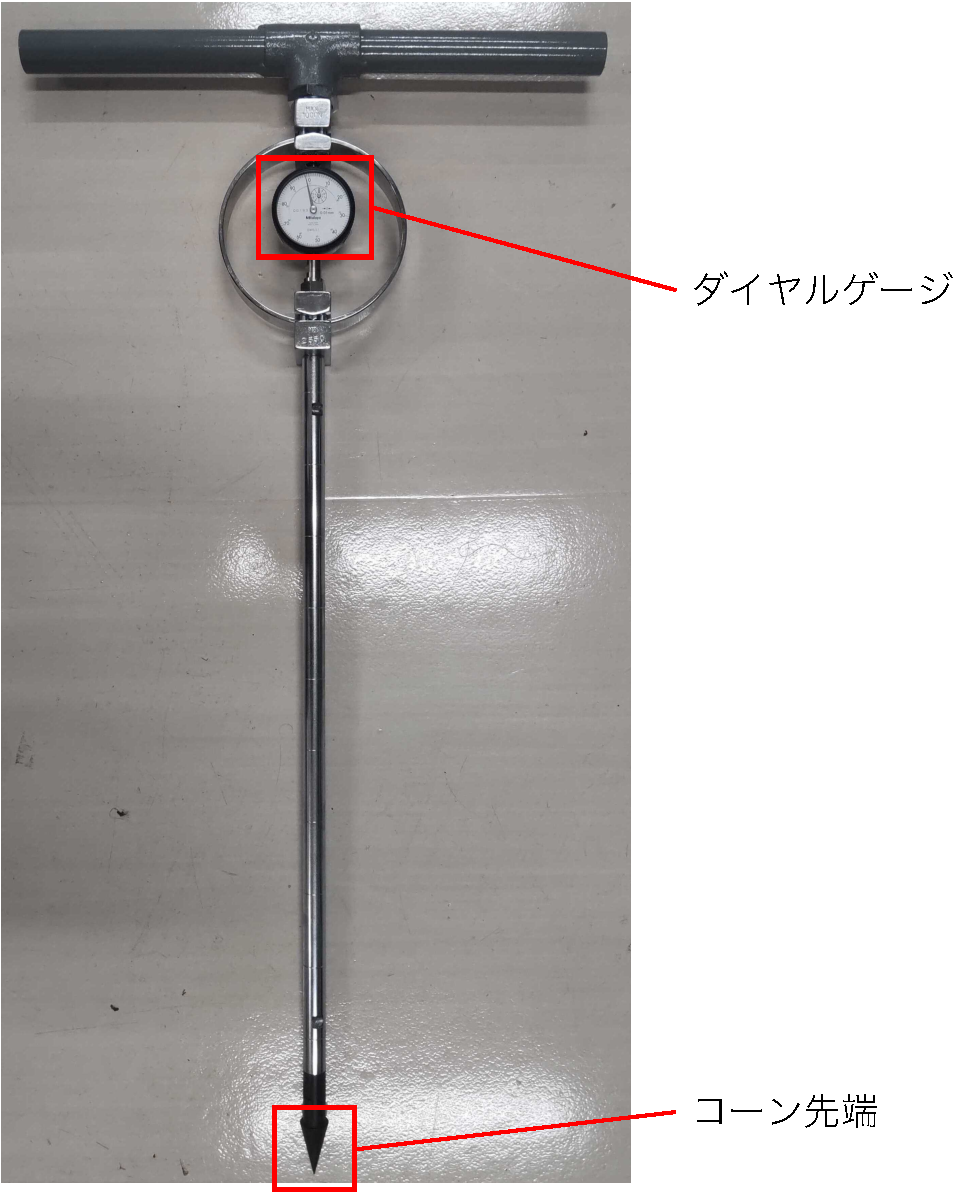
\includegraphics[keepaspectratio, width=0.5 \linewidth]{cone_penetrometer.pdf}
    \caption{コーンペネトロメータ}
    \label{fig:cone_penetrometer}
\end{figure}

\vspace{3\zh}
\begin{table}[t]
    \caption{走行に必要なコーン指数(\protect \citeja{maff2015}を基に作成)}
    \label{tab:traffic_cone_index}
    \centering
    \begin{tabular}{cc}
        \toprule
        建設機械の種類                      & コーン指数[\si{\kN/\m^2}] \\
        \midrule
        超湿地ブルドーザー                    & 200以上                \\
        湿地ブルドーザー                     & 300以上                \\
        普通ブルドーザー(\SI{15}{\tonne}級程度) & 500以上                \\
        普通ブルドーザー(\SI{21}{\tonne}級程度) & 700以上                \\
        スクレープドーザ                     & 600以上                \\
                                     & (超湿地型は400以上)         \\
        被けん引式スクレーパ(小型)               & 700以上                \\
        自走式スクレーパ(小型)                 & 1,000以上              \\
        ダンプトラック                      & 1,200以上              \\
        \bottomrule
    \end{tabular}
\end{table}
\clearpage

\subsection{地盤強度の間接推定}
\label{subsec:intro_presearch_indirect}

\end{document}